%
% Presentation: Analysing Debian packages with Neo4j
% Author: Norbert Preining
% Copyright: 2017 Norbert Preining
% License: GPL3+
%
\documentclass[hyperref]{beamer}
\usefonttheme{serif}
\usefonttheme{professionalfonts}
\hypersetup{pdfencoding=auto}
\usepackage{url,graphicx}
\usepackage{fontspec,unicode-math}
\defaultfontfeatures{Scale=0.95,Numbers=OldStyle}
\unimathsetup{math-style=ISO,mathup=sym}
\setmainfont{Lucida Bright OT}[%
  ItalicFont=Lucida Bright OT Italic,
  BoldFont=Lucida Bright OT Demibold,
  BoldItalicFont=Lucida Bright OT Demibold Italic,
  Ligatures=TeX]
\setsansfont{Lucida Sans OT}[%
  ItalicFont=Lucida Sans OT Italic,
  BoldFont=Lucida Sans OT Demibold,
  BoldItalicFont=Lucida Sans OT Demibold Italic,
  Ligatures=TeX]
\setmonofont{Lucida Grande Mono DK}[%
  ItalicFont=Lucida Grande Mono DK Italic,
  BoldFont=Lucida Grande Mono DK Bold,
  BoldItalicFont=Lucida Grande Mono DK Bold Italic,
  ]
\setmathfont{Lucida Bright Math OT}[%
  RawFeature=+ss04]
\setmathfont{Lucida Bright Math OT Demibold}[%
  version=bold,
  RawFeature=+ss04]

\usepackage{listings}
\lstset{%
  backgroundcolor=\color{lightgray},basicstyle={\ttfamily\small},showspaces=false}


\pgfdeclareimage[width=2cm]{accelia}{accelia-large.png}
\logo{\pgfuseimage{accelia}}

\newcommand{\acro}[1]{\textsc{\MakeLowercase{#1}}}
\newcommand\img[4]{%
  \bgroup%
  \setbox0=\hbox{\hskip #3\vbox to 0pt{\vskip #4 \includegraphics[height=#2]{#1}}}%
  \dp0=0pt %
  \ht0=0pt %
  \wd0=0pt %
  %\hbox to \textwidth{\hfill\hbox{\box0}}%
  \hbox{\box0}
  \egroup}

\setbeamertemplate{sidebar right}{%
  \vskip5pt%
  \llap{\insertlogo\hskip0.1cm}%
  \vfill
}
  

\setbeamertemplate{navigation symbols}{}
\newcommand{\itemvisible}{\setbeamercovered{transparent=30}}
\newcommand{\iteminvisible}{\setbeamercovered{transparent=100}}



\newcommand{\cutin}[1]{%
\begin{frame}[c]\begin{center}{\Large\bf\color{myblue}#1}\end{center}\end{frame}}
\definecolor{myblue}{rgb}{0.0,0.0,0.7}
\def\cred{\color{red}}
\def\cblue{\color{myblue}}
\def\sis{\\[\smallskipamount]}
\def\mis{\\[\medskipamount]}
\def\bis{\\[\bigskipamount]}

\author{Norbert Preining\\
{\small\url{http://www.preining.info/}}}
\institute{%
  \begin{minipage}{0.4\linewidth}\centering
    \includegraphics[width=3cm]{accelia-v.png}\\
    Tokyo, Japan\
    \url{http://www.accelia.net/}
  \end{minipage}
  \qquad
  \begin{minipage}{0.3\linewidth}\centering
    
\includegraphics[width=1cm]{debian-open-logo.png}\\
    Debian Developer
  \end{minipage}
}

\title{Analysing Debian packages with Neo4j}
\date{2017-10-19}
\begin{document}
\begin{frame}
  \maketitle
\end{frame}

\begin{frame}
  \frametitle{Self introduction}
  \begin{itemize}
  \item Logician by education, 20+ years in research on Theoretical
    Computer Science and Mathematical Logic at various universities\bis
  \item Since one year working at Accelia Inc. (\acro{CDN}/\acro{IT} Service) on
    security and machine learning\bis
  \item Debian Developer since about 20 years, mainly responsible for
    \TeX\ related packages\bis
  \item Developer of \TeX\ Live, main author of \TeX\ Live Manager and
    installer 
  \end{itemize}
\end{frame}

\begin{frame}
  \frametitle{Why graph database?}
  \begin{itemize}
  \item Preparing a recommender system for potential clients\bis
  \item Natural way to represent the available data\bis
  \item Learning something new\bis
  \item Highly non-hierarchical data in graph database (many examples
    have a clear hierarchical structure)\bis
  \item Reasonable sized (not too small) and meaningful content\bis
    \pause
  \item Hip!(?)\bis
  \end{itemize}
\end{frame}

\begin{frame}
  \frametitle{Overview}
  \begin{itemize}
  \item Quick introduction to Debian\bis
  \item Packages in Debian\bis
  \item Ultimate Debian Database\bis
  \item Representing packages as a graph (``Database schema'')\bis
  \item Conversion from \acro{UDD} to Neo4j\bis
  \item Sample queries and visualizations\bis
  \item Concluding remarks
  \end{itemize}
\end{frame}

\cutin{Introduction to Debian}

\begin{frame}
  \frametitle{Debian}
  \begin{itemize}
  \item Open source Linux distribution\bis
  \item Developed (mostly) by volunteers\bis
  \item Lots of offspring (e.g.\ Ubuntu)\bis
  \item Strict license requirements (\acro{DFSG})\bis
  \item About 31000 source packages building about 82000 binary packages
  \end{itemize}
\end{frame}

\begin{frame}
  \frametitle{Debian releases}
  \begin{block}{Stable}
    officially released, security support and updates
  \end{block}

  \pause
  \begin{block}{Testing}
    preparation for the next stable
  \end{block}

  \pause
  \begin{block}{Development (sid)}
    entrance point for all packages, main development place
  \end{block}

  \pause
  \begin{block}{Experimental}
    what it says, for testing, often used during pre-release freeze
  \end{block}
  \pause
  Other releases: point releases for stable, oldstable, historic releases
\end{frame}

\begin{frame}

  \img{debian-update-jessie-stretch-buster-12-638.png}{8cm}{-0.5cm}{0cm}

  \hbox{~}
  \vfill
  \vspace{6cm}
  Image by Youhei Sasaki (\acro{CC-NC-SA})
\end{frame}

\cutin{Packages in Debian}

\begin{frame}
  \frametitle{Packages}
  \begin{itemize}
  \item source packages and binary packages\bis
  \item Developer uploads source package (and his own's arch binary
    package, or source-only upload)\bis
  \item other architectures are built by auto-builders\bis
  \item upload is included in unstable (or rejected)
  \end{itemize}
\end{frame}

\begin{frame}
  \vspace{-0.5cm}
  \begin{center}
    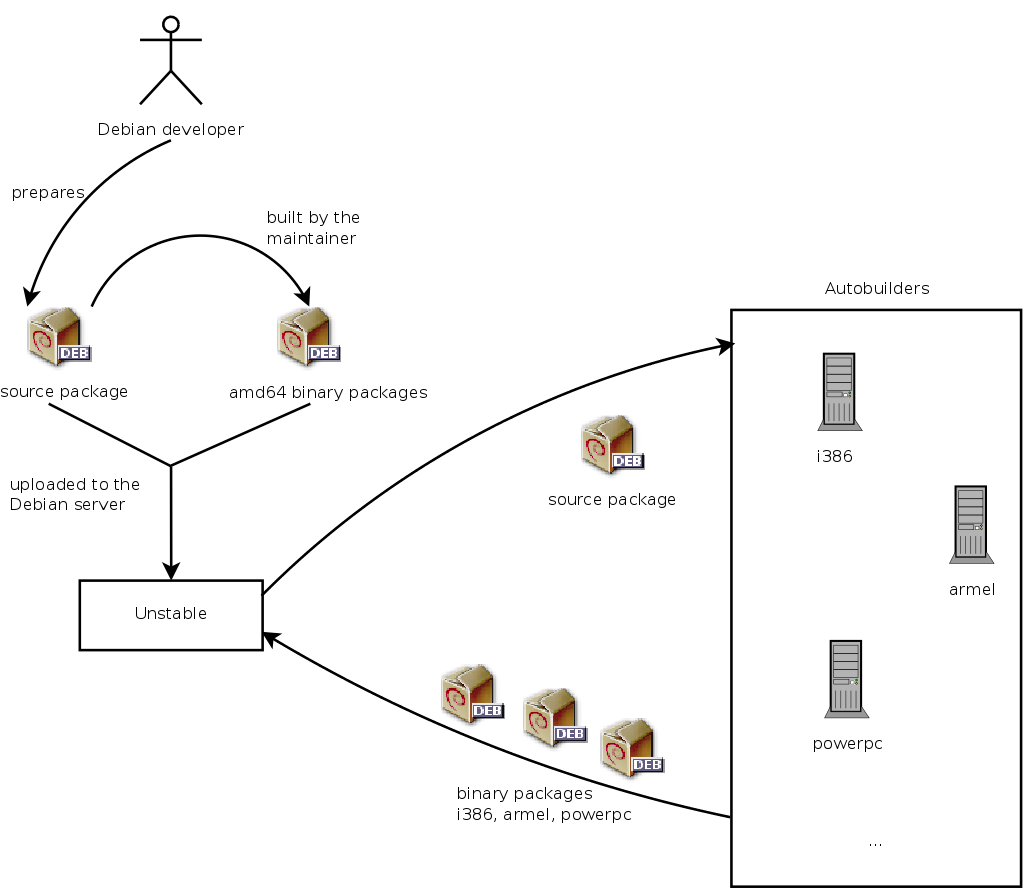
\includegraphics[height=0.9\textheight]{autobuilder.png}
  \end{center}
  \vspace{-2cm}
  \small Debian Administrator's\\
  Handbook, \acro{GPL}
\end{frame}

\begin{frame}
  \frametitle{Versions of packages in Debian}
  \begin{itemize}
  \item current versions in sid, testing, stable, oldstable, security
    releases\bis
  \item intermediate versions that did not end up in a release
  \end{itemize}
  \begin{block}{Example}
    \texttt{asymptote} package:\\
    oldstable: 2.31-2, stable: 2.38-2, testing and sid: 2.41-2

    other versions uploaded to unstable: 2.35-1, 2.35-2, 2.37-1,
    2.38-1, 2.41-1, \ldots
  \end{block}
\end{frame}

\begin{frame}
  \frametitle{Version numbers}
  \begin{center}
    [epoch:]upstream\_version[-debian\_revision] 
  \end{center}
  \begin{block}{Examples}
    asymptote 2.41-2:\\
    \hspace{1em}upstream\_version: 2.41\\
    \hspace{1em}debian\_release: 2

    \medskip\pause
    musixtex 1:1.20.ctan20151216-4:\\
    \hspace{1em} epoch: 1\\
    \hspace{1em} upstream\_version: 1.20.ctan20151216\\
    \hspace{1em} debian\_release: 4
  \end{block}
\end{frame}

\begin{frame}
  \frametitle{Components of a package}
  \begin{itemize}
  \item Maintainer: who is responsible\bis
  \item Uploaders: who is allowed to upload packages\bis
  \item Section, Priority: relevant for structuring the huge set of
    packages\bis
  \item Version\bis
  \item dependency declarations\bis
  \item lots of further fields
  \end{itemize}
\end{frame}

\begin{frame}
  \frametitle{Some caveats}
  \begin{itemize}
  \item one source package can build many different binary
    packages\bis 
  \item the names of source package and binary package are not
    necessary the same (necessarily different when building multiple
    binary packages)\bis
  \item binary packages of the same name (but different version) can
    be built from different source packages
  \end{itemize}
\end{frame}

\begin{frame}
  \frametitle{Dependencies}
  \begin{block}{for source packages}
    Build-Depends, Build-Depends-Indep, Build-Depends-Arch,
    Build-Conflicts, Build-Conflicts-Indep, Build-Conflicts-Arch 
  \end{block}

  \begin{block}{for binary packages}
    Depends, Pre-Depends, Recommends, Suggests, Enhances, Breaks, Conflicts
  \end{block}

  \begin{block}{various formats of dependencies}
    \texttt{Relation: pkg}\\
    \texttt{Relation: pkg (<< version)}\\
    \texttt{Relation: pkg | pkg}\\
    \texttt{Relation: pkg [arch1 arch2]}
  \end{block}
\end{frame}

\cutin{Ultimate Debian Database \acro{UDD}}
\begin{frame}
  \frametitle{The \acro{UDD}}
  Imports data from a variety of sources:
  \begin{itemize}
  \item packages and source files, from both Debian and Ubuntu\mis
  \item bugs from the Debian \acro{BTS}\mis
  \item popularity contest\mis
  \item history of uploads\mis
  \item history of migrations\mis
  \item lintian (conformance check tool)\mis
  \item orphaned packages\mis
  \item debtags, carnivore, Ubuntu bugs, \acro{NEW} queue, \acro{DDTP}
    translations, \ldots
  \end{itemize}
\end{frame}

\cutin{The \acro{UDD} schemata\\[12pt]
  \normalfont
  \url{https://udd.debian.org/schema/}}

\begin{frame}
  \frametitle{\acro{UDD} schemata}
  \begin{itemize}
  \item highly de-normalized\bis
  \item good example of grown-over-time schemata\bis
  \item lots of duplication without connections\bis\pause
  \item a pleasure for any SQL fetishist ;-)
  \end{itemize}
\end{frame}

\cutin{Can we put the \acro{UDD} into a Graph Database?}

\begin{frame}
  \frametitle{Entities: first steps: source and binary packages}
  \begin{block}{source builds binary relation}
    Use different node types for (versioned) source and binary
    package; link increasing versions
  \end{block}

  \pause
  \begin{block}{unversioned dependencies}
    Use different node types for unversioned and versioned source and
    binary packages
  \end{block}

  \pause
  \begin{block}{Node and relations (for now)}
    Nodes: \texttt{sp} (source package), \texttt{vsp} versioned source
    packages, \texttt{bp} (binary package), \texttt{vbp} versioned
    binary package

    \medskip
    \begin{center}
      \texttt{vsp -[:is\_instance\_of]-> sp}\\
      \texttt{vbp -[:is\_instance\_of]-> bp}\\
      \texttt{sp -[:builds]-> bp}\\
      \texttt{vbp -[:next]-> vbp}\\
      \texttt{vsp -[:next]-> vsp}\\
    \end{center}
  \end{block}
\end{frame}

\begin{frame}
  \begin{center}
    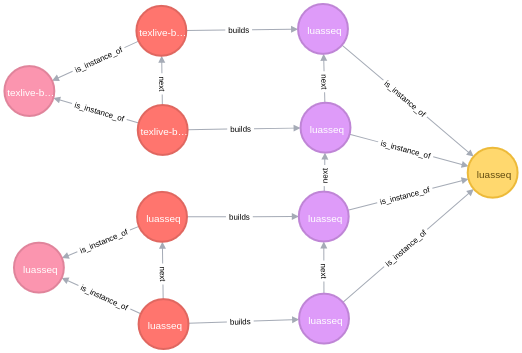
\includegraphics[height=7cm]{simple-graph.png}
  \end{center}
\end{frame}

\begin{frame}
  \frametitle{Suites}

  Register the binary packages that are included in a suite (release):

  \bigskip
  Node type: \texttt{suite}

  \bigskip
  \begin{center}
     \texttt{suite -[:contains]-> vbp}
  \end{center}
\end{frame}

\begin{frame}
  \begin{center}
    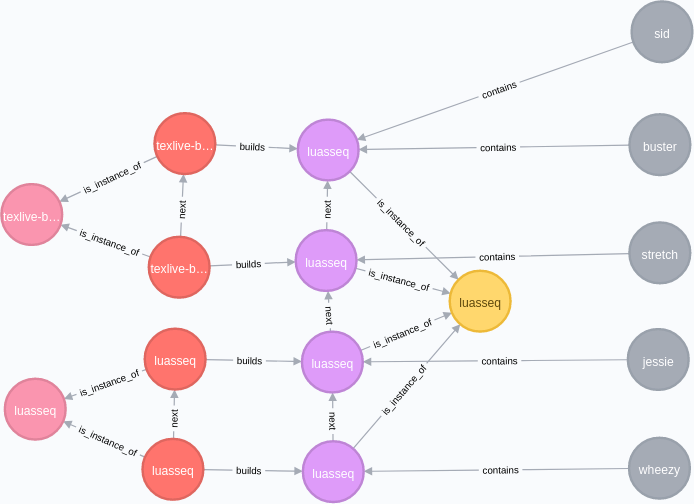
\includegraphics[height=7cm]{add-releases.png}
  \end{center}
\end{frame}

\begin{frame}
  \frametitle{Maintainers}

  Register the maintainers of binary and source packages:
  
  \bigskip
  Node type: \texttt{mnt}

  \bigskip
  \begin{center}
     \texttt{mnt -[:maintains]-> vbp}\\
     \texttt{mnt -[:maintains]-> vsp}
  \end{center}
\end{frame}

\begin{frame}
  \begin{center}
    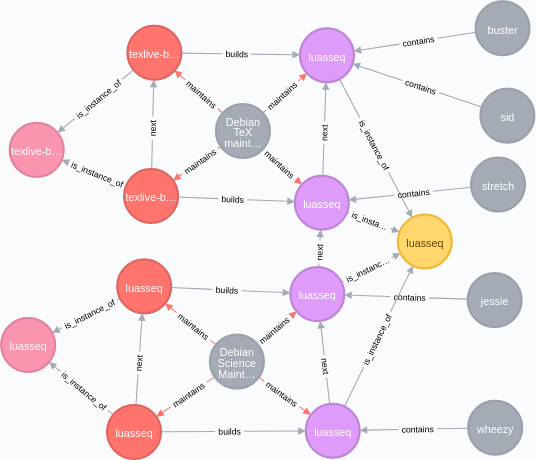
\includegraphics[height=7cm]{add-maintainer.png}
  \end{center}
\end{frame}

\begin{frame}
  \frametitle{Dependencies}
  Current state: dependency is represented as relation between a
  versioned (source/binary) package and \emph{unversioned} binary
  package with additional properties (type of relation, version
  number)

  \begin{center}
    \texttt{vbp -[:depends {reltype: TYPE, relversion: VERS}]-> bp}
  \end{center}
  Where \texttt{TYPE} is one of \texttt{<<}, \texttt{<=}, \texttt{==},
  \texttt{>=}, \texttt{>>}.

  If it is an \emph{unversioned} relation \texttt{TYPE} is
  \texttt{none}, and \texttt{relversion} is 1.
\end{frame}

\begin{frame}
  \begin{center}
    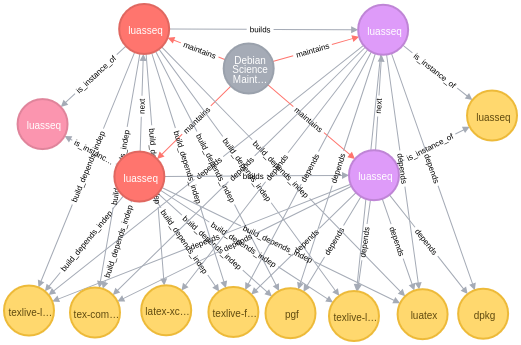
\includegraphics[height=7cm]{add-depends.png}
  \end{center}
\end{frame}

\begin{frame}
  \frametitle{Alternative dependencies}
  Add a new node type \texttt{altdep} and a new relation
  \texttt{is\_satisfied\_by}.
  \begin{center}
    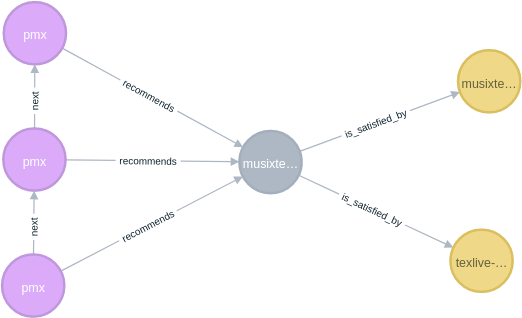
\includegraphics[height=5cm]{altdeps.png}
  \end{center}
  \texttt{name} of the \texttt{altdep}:\\
  \texttt{musixtex (>= 1:0.98-1) | texlive-music}
\end{frame}

\cutin{Summary of Nodes and Relations}

\begin{frame}
  \frametitle{Nodes and relations}
  \begin{block}{Nodes and attributes}
    \begin{itemize}
    \item \texttt{mnt}: \texttt{name}, \texttt{email}
    \item \texttt{bp}, \texttt{sp}, \texttt{suite}, \texttt{altdeps}: \texttt{name}
    \item \texttt{vbp}, \texttt{vsp}: \texttt{name}, \texttt{version}
    \end{itemize}
  \end{block}

  \begin{block}{Relations and attributes}
    \begin{itemize}
    \item \texttt{breaks}, \texttt{build\_conflicts},
      \texttt{build\_conflicts\_indep}, \texttt{build\_depends},
      \texttt{build\_depends\_indep}, \texttt{conflicts},
      \texttt{depends}, \texttt{enhances}, \texttt{is\_satisfied\_by},
      \texttt{pre\_depends}, \texttt{provides}, \texttt{recommends}, 
      \texttt{replaces}, \texttt{suggests}:\\
      Attributes: \texttt{reltype}, \texttt{relversion}
    \item \texttt{builds}, \texttt{contains},
      \texttt{is\_instance\_of}, \texttt{maintains}, \texttt{next}: no attributes
    \end{itemize}
  \end{block}
\end{frame}

\begin{frame}
  \frametitle{Number of entities}
  \begin{block}{Nodes}
    suite: 27, mnt: 3492, altdeps: 8729, sp: 31465, bp: 145284, vsp:
    78783, vbp: 235534

    \bigskip
    Total: 503316
  \end{block}

  \begin{block}{Relations}
    breaks:~48843, build\_conflicts:~3331,
    build\_conflicts\_indep:~42, build\_depends:~559374,
    build\_depends\_indep:~96780, builds:~223458, conflicts:~42956,
    contains:~354899, depends:~1729800, enhances:~5981,
    is\_instance\_of:~314317, is\_satisfied\_by:~22231,
    maintains:~314317, next:~152844, pre\_depends:~12091,
    provides:~100067, recommends:~92607, replaces:~62758,
    suggests:~112001

    \bigskip
    Total: 4248696
  \end{block}
\end{frame}

\cutin{Conversion from \acro{UDD} to Neo4j}

\begin{frame}[fragile]
  \frametitle{Conversion step 1: Getting the data}
  \begin{itemize}
  \item \acro{UDD} has a public mirror:
    \url{public-udd-mirror.xvm.mit.edu}\bis
  \item Postgresql DB, use \texttt{psql} to get the various tables in
    \texttt{csv} format
  \end{itemize}
  \begin{lstlisting}
export PGPASSWORD='public-udd-mirror'
psql -P pager=off --host=public-udd-mirror.xvm.mit.edu \
  --user=public-udd-mirror udd <<'EOF'
\pset format unaligned
\pset fieldsep '\t'
\pset footer off
\o sources.csv
select * from sources ;
\o packages.csv
select * from packages ;
EOF
\end{lstlisting}
\end{frame}

\begin{frame}[fragile]
  \frametitle{Conversion step 2: Into Neo4j}
  My first try was generating Cypher statements \ldots\ lots of them.

  \pause That was not really good ;-)\pause

  \begin{block}{Use \texttt{neo4j-import} tool}
    \begin{itemize}
    \item generate for each node/relation a \texttt{csv} with ids
    \item run \texttt{neo4j-import}, takes a few seconds!
    \end{itemize}
  \end{block}
  \pause
  \begin{lstlisting}
$ neo4j-import ...
...
IMPORT DONE in 11s 162ms. 
Imported:
  503316 nodes
  4248696 relationships
  7102164 properties
Peak memory usage: 521.04 MB
\end{lstlisting}
\end{frame}

% $ faked to fix above miss

\begin{frame}
  \frametitle{How to generate node/relation csv?}
  \begin{itemize}
  \item Perl program parsing the \texttt{csv} files from psql\bis
  \item generates a huge hash with all information (in fact more than
    currently evaluated)\bis
  \item for each item generated a unique \acro{UUID}\bis
  \item generates the necessary \texttt{csv} files
  \end{itemize}

  \medskip
  \pause
  Warning: the script needs currently about 16G of memory. Killed my
  laptop a few times.
\end{frame}

\cutin{Sample queries}

\begin{frame}[fragile]
  \frametitle{Checking build-deps}

  Find all packages in Jessie that build depends on some version of
  \texttt{tex-common}:

\begin{lstlisting}
match (BP:bp)<-[:build_depends]-(VSP:vsp)-[:builds]->
  (VBP:vbp)<-[:contains]-(S:suite)
  where BP.name="tex-common" and S.name="jessie"
  return BP, VSP, VBP, S
\end{lstlisting}
\pause
\begin{center}
  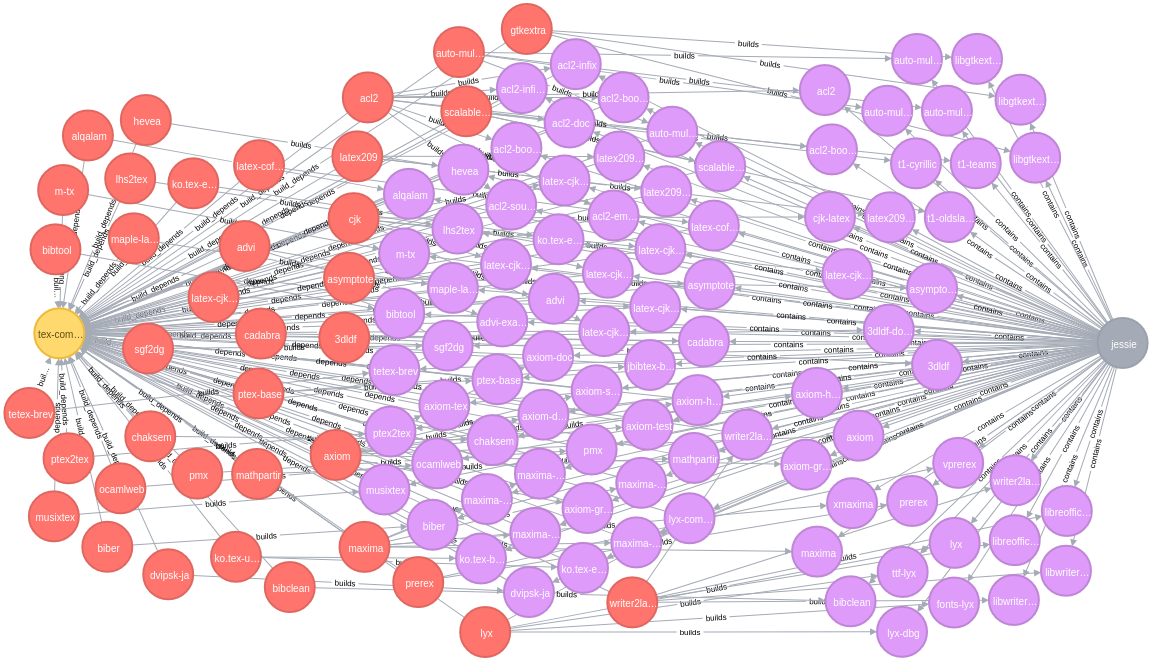
\includegraphics[height=4cm]{bd-on-tex-common.png}
\end{center}
\end{frame}

\begin{frame}[fragile]
  \frametitle{Most depend on package in sid}
  Number of packages in sid that build depend on $X$, ordered by
  number of depending packages
  \begin{lstlisting}
 match (S:suite)-[:contains]->(VBP:vbp)-[:builds]-
  (VSP:vsp)-[:build_depends]-(X:bp) 
  where S.name = "sid" 
  with X.name as pkg,count(VSP) as cntr 
    return pkg,cntr order by -cntr
\end{lstlisting}
\pause
gives: debhelper: 54938, pkg-config: 9000, dh-python: 8930
\end{frame}

\cutin{Conclusions}

\begin{frame}
  \frametitle{Lessons learned}
  \begin{itemize}
  \item Finding a good representation is tricky -- see below for
    future work\bis
  \item Don't use Cypher for importing any reasonable amount of
    data\bis
  \item Conversion from an old/grown RDB is a pain\bis
  \item Starting from scratch for a new application is fun\bis
  \item Visualization in Chrome/Firefox is often a pain -- depending
    on version and OS either the one or the other is better (why? no
    idea!) 
  \end{itemize}
\end{frame}

\begin{frame}
  \frametitle{Future work -- time allowing}
  \begin{itemize}
  \item Include the bug database
  \item Include also intermediate releases by parsing the \acro{UDD}
    table for uploads
  \item Rework dependency management\\
    I don't like the current status: I would prefer if the dependency
    points into the tree of \texttt{vbp} and has only an attribute for
    the relation type.
  \item After all that, rewrite the \acro{UDD} dashboard and see how
    far it simplifies the \acro{SQL} code.
  \item More graph theoretic: find dependency cycles, connected
    components etc
  \end{itemize}
\end{frame}

\begin{frame}
  \frametitle{Sources}
  Sources for the scripts as well as the slides are available on the
  Github project:
  \begin{center}
    \url{https://github.com/norbusan/debian-graph}
  \end{center}

  \pause
  \begin{center}
    Thanks for the attention
  \end{center}
\end{frame}
\end{document}

